\chapter{Элементы физики сверхпроводящих квантовых цепей} \label{c1}

В Главе \ref{c1} кратко излагаются элементы физики сверхпроводимости, СКЦ и квантовой оптики, необходимые для изложения и обсуждения результатов диссертационной работы. Вначале кратко описываются причины возникновения сверхпроводимости и изгалаются основные физические свойства сверхпроводника. Затем подробно рассматривается эффект Джозефсона в туннельном SIS-переходе, описываются основные модели описания эффекта Джозефсона приводятся основные свойства такого SIS-перехода (далее называемого джозефсоновским переходом) в различных режимах работы. Делается вывод о том, почему джозефсоновский переход находит широкое применение в классической и квантовой сверхпроводящей электронике. Описывается общий формализм квантования сверхпроводящей электрической цепи и рассчитываются параметры некоторых видов СКЦ --- потоковый кубит, трансмон, а также rf-SQUID. 
Отдельный раздел посвящен элементам квантовой оптики --- науки, которая описывает квантование электромагнитного поля и эффекты взаимодействия такого поля с атомами и молекулами. 
\section{Обзор явления сверхпроводимости} \label{s1_sc_phys}
Явление сверхпроводимости было открыто в 1911 г. в лаборатории Х. Камерлинг-Оннеса, и практически сразу началось интенсивное как теоретическое, так и экспериментальное изучение данного явления. Оказалось, что некоторые металлы при температурах $T<T_c$ демонстрируют целый ряд необычных физических свойств. Опуская подробности, перечислим наиболее интересные свойства сверхпроводников:
\begin{enumerate}
	\item Полное отсутствие сопротивления электрическому току;
	\item Полное вытеснение магнитного поля из объема сверхпроводника (эффект Мейсснера);
	\item Квантование магнитного потока через замкнутый контур из сверхпроводящего металла;
	\item Скачкообразное возрастание теплоемкости металла при переходе через $T_c$.
\end{enumerate}	
Объяснить поведение сверхпроводников на феноменологическом уровне удалось с помощью классической теории Лондонов, которая опирается на двухжидкостную модель электронов в металле: часть электронов предполагаются <<сверхпроводящими>>, т.е. способными переносить электрический ток в отсутствие внешнего электрического поля. Одного этого предположения практически достаточно для того, чтоб объяснить многие свойства сверхпроводников, в частности, идеальный диамагнетизм. Квантовое обобщение этой теории было построено Гинзбургом и Ландау на основе теории фазовых переходов II рода. Ключевым предположением теории ГЛ было введение общей волновой функции сверхпроводящих электронов $\Psi = |\Psi(\mathbf{r})| e^{i\varphi({\mathbf{r}})}$ в металле и её рассмотрение в качестве параметра порядка, характеризующего фазовый переход. Некоторые вопросы, на которые теория Лондонов давала качественно неправильный ответ (например, значение поверхностной энергии границы между нормальной и сверхпроводящей фазами), были верно описаны с помощью теории ГЛ. Строго говоря, эта теория применима для описания сверхпроводимости в случае $T_c-T \ll T_c$\footnote[1]{Имеется также ограничение применимости теории, связанное с тем, что при $T$ очень близком к $T_c$ становятся важными флуктуационные эффекты.}, но оказывается, что для многих практически важных задач решение на основе теории ГЛ качественно совпадает с выводами микроскопической теории сверхпроводимости.

Несмотря на значительный прогресс в объяснении многих эксперименальных свойств сверхпроводников, истинный механизм возникновения сверхпроводимости долгое время оставался неописанным. Одним из результатов, указавшим на причину сверхпроводимости, стал изотопический эффект: для различных изотопов сверхпроводника в эксперименте наблюдается соотношение $T_c \cdot M^{\alpha}=\text{const}$. Следовательно, сверхпроводимость возникает из-за взаимодействия электронов с кристаллической решеткой. При детальном теоретическом анализе было выявлено, что возможен процесс эффективного притяжения электронов друг к другу посредством обмена фононами. В 1957 Купер \cite{CooperPairs} показал, что даже малое отрицательное (притягивающее) взаимодействие между электронами дает очень необычный результат. Состояние металла, в котором все электроны занимают состояния с $E<E_F$, даже при $T=0$ не является основным. В металле могут возникать определенного рода парные возбуждения, при которых два электрона с противоположными квазиимпульсами и спинами занимают состояния с энергией $E\approx E_F\! +\! \Delta$, где $\Delta$ --- некоторая константа, зависящая от температуры. Такие возбуждения называются \textit{куперовскими парами}, и их образование оказывается энергетически выгодным.  В 1958 г. Бардин, Купер и Шриффер \cite{Bardeen} нашли явный вид волновой функции основного состояния  и посчитали его энергию. Оказалось, что полная энергия состояния с некоторым количеством куперовских пар оказывается меньше по сравнению с энергией состояния металла без пар, на величину порядка $N(0)\Delta^2$. Параметр $\Delta$ определяется характером электрон-фононного взаимодействия. Его значение определяет критическую температуру: $\Delta = 1.76 k_b T_c$, среднее количество куперовских пар в металле: $\Delta N(0) \approx k_b T_c/E_F$, и кроме того, является средней энергей связи в паре в расчете на один электрон. По этой причине $\Delta$ называется \textit{энергетической щелью}: для разрыва куперовской пары необходимо затратить энергию $2\Delta$, при этом пара распадается на два квазичастичных возбуждения. Волновую функцию основного состояния пар в БКШ-теории можно записать как \cite{Tinkham}:
\begin{equation}
\ket{\psi_\varphi} = \prod_{\vec{k}}^{}(|u_{\vec{k}}|+|\nu_{\vec{k}}|e^{i\varphi}c^\dag_{\vec{k},\uparrow}c^\dagger_{-\vec{k}, \downarrow})\ket{\phi_0}.
\end{equation}  
Чрезвычайно важным обстоятельством является наличие фазового множителя при амплитуде вероятности рождения куперовской пары $|\nu_{\vec{k}}|$. Фаза $\varphi$ одна и та же для каждой пары и иллюстрирует то факт, что спаренные электроны образуют единое квантовое состояние. Для объемного сверхпроводника эта фаза не зависит от координаты. Можно показать, что в состоянии $\ket{\psi_\varphi}$ полное число пар не определено, однако, относительная дисперсия стремится к нулю по мере увеличения среднего числа электронов в системе, поэтому такое приближение можно считать разумным. Из состояний с $\ket{\psi_\varphi}$ c различными фазами можно получить состояние с определённым числом куперовских пар $\ket{\psi_n}$. Для этого достаточно заметить, что слагаемые в состояние $\ket{\psi_\varphi}$, отвечающие числу пар $N$ имеют фазовый множитель $e^{in{\varphi}}$, и при усреднении по фазам все остальные слагаемые дадут нулевой вклад:
\begin{equation}
\ket{\psi_n} = \int_{0}^{2 \pi}e^{-i n \varphi} \ket{\psi_\varphi}.
\end{equation} 
Соотношение между $\ket{\psi_\varphi}$ и $\ket{\psi_n}$ имеет такой же вид, как и для векторов состояния $\ket{x}$~и~$\ket{p}$ свободной частицы, то есть, $n$ и $\varphi$ в сверхпроводнике являются канонически сопряженными переменными. Для них можно вывести коммутационное соотношение $[\hat{n}, \hat{\varphi}]=-i$ и соотношение неопределенностей $\Delta\varphi \cdot \Delta n \approx \hbar$. Таким образом, изолированный остров сверхпроводника обладает макроскопической квантовой степенью свободы: фаза играет роль координаты, а число куперовских пар --- роль импульса. Ясно, что если остров находится при $T\!=\!0$ и полностью изолирован от других островов, то $N$ фиксировано, а значит $\phi$ полностью неопределена и не имеет физического смысла. Но оказывается, что в системе из нескольких островов возможны более нетривиальные ситуации, когда имеет смысл говорить о суперпозициях состояний с разными значениями заряда $\hat{Q}\! = \!2e\hat{N}$. Квантование степени свободы, которая сама по себе формулируется в терминах существенно квантовых переменных: числа пар и фазы волновой функции --- представляет из себя достаточно нетривиальную задачу. Поэтому оставим этот вопрос немного в стороне и для начала проясним, как фаза и число (суммарный заряд) куперовских пар могут проявлять себя в эксперименте. 

В некоторых случаях глобальная фаза сверхпроводника проявляется на макроскопическом уровне. Такие ситуации особенно интересны, поскольку позволяют наблюдать квантовые эффекты в сверхпроводниках при непосредственном измерении макроскопических величин. Например, экранирование внешнего магнитного поля в неодносвязном сверхпроводнике (кольце) приводит к тому, что магнитный поток проникает в полости дискретными порциями --- квантами потока. Также существует способ привести два различных сверхпроводника в контакт, так чтобы каждый из них <<чувствовал>> фазу соседнего. Оказывается, что при этом сила тока и падение напряжения на этом контакте однозначно определяются соотношением фаз между двумя сверхпроводящими берегами. Перейдём к рассмотрению этих двух задач и опишем явления, известные под названием \textit{квантование магнитного потока} и \textit{эффект Джозефсона}
\section{Квантование магнитного потока}
Чтобы глубже осознать суть эффекта Джозефсона, рассмотрим вначале эффект квантования магнитного потока.
Глобальная фаза необычно проявляет себя при рассмотрении неодносвязного сверхпроводника, например, кольца индуктивности $L$, помещенного во внешнее магнитное поле $\vec{B}$. Поле создаёт некоторый магнитный поток через кольцо $\Phi_{ext}$. Также поле проникает в тонкий поверхностный слой порядка $\lambda$, и в этом слое сверхпроводника возникает экранирующий (мейсснеровский) ток $I_m$. Воспользуемся вторым уравнением теории ГЛ, согласно которому:
\begin{equation}
\mathbf{j_m} = \frac{|\Psi|^2}{\lambda^2}\big(\frac{\hbar c}{2e}\mathbf{\nabla}\varphi-\mathbf{A}\big)
\label{eq:2GL}
\end{equation} 
Выберем некоторый контур $\mathcal{L}$, замкнутый вокруг отверстия и проходящий в глубине кольца. Тогда вдоль этого контура $\mathbf{j_m}=0$, и полный магнитный поток $\Phi\!=\!LI_m\!+\!\Phi_{ext}$ можно записать как:
\begin{equation}
\Phi = \oint\displaylimits_{\mathcal{L}}^{} \mathbf{A} d\boldsymbol{\ell} = \frac{\hbar c}{2e}\oint\displaylimits_{\mathcal{L}}^{} \nabla\varphi d\boldsymbol{\ell}.
\label{eq: 2GL}
\end{equation}
Полное изменение фазы вдоль контура может составлять только величину, кратную $2\pi$, поскольку волновая функция обязана быть однозначной, см. также Рис.~\ref{img:coils}. Получаемое выражение
\begin{equation}
\Phi = \frac{\hbar c}{2e} \cdot 2\pi N = N\Phi_0
\label{eq: flux_q}
\end{equation}
означает, что магнитный поток в кольце квантуется, т.е. принимает значения кратные величине $\Phi_0={hc}/{2e}$, называемой \textit{квантом магнитного потока}. Значение $\Phi_0$ составляет $2.067\cdot10^{-15}$~Вб в единицах СИ. 	
\begin{figure}[ht] 
	\centering
	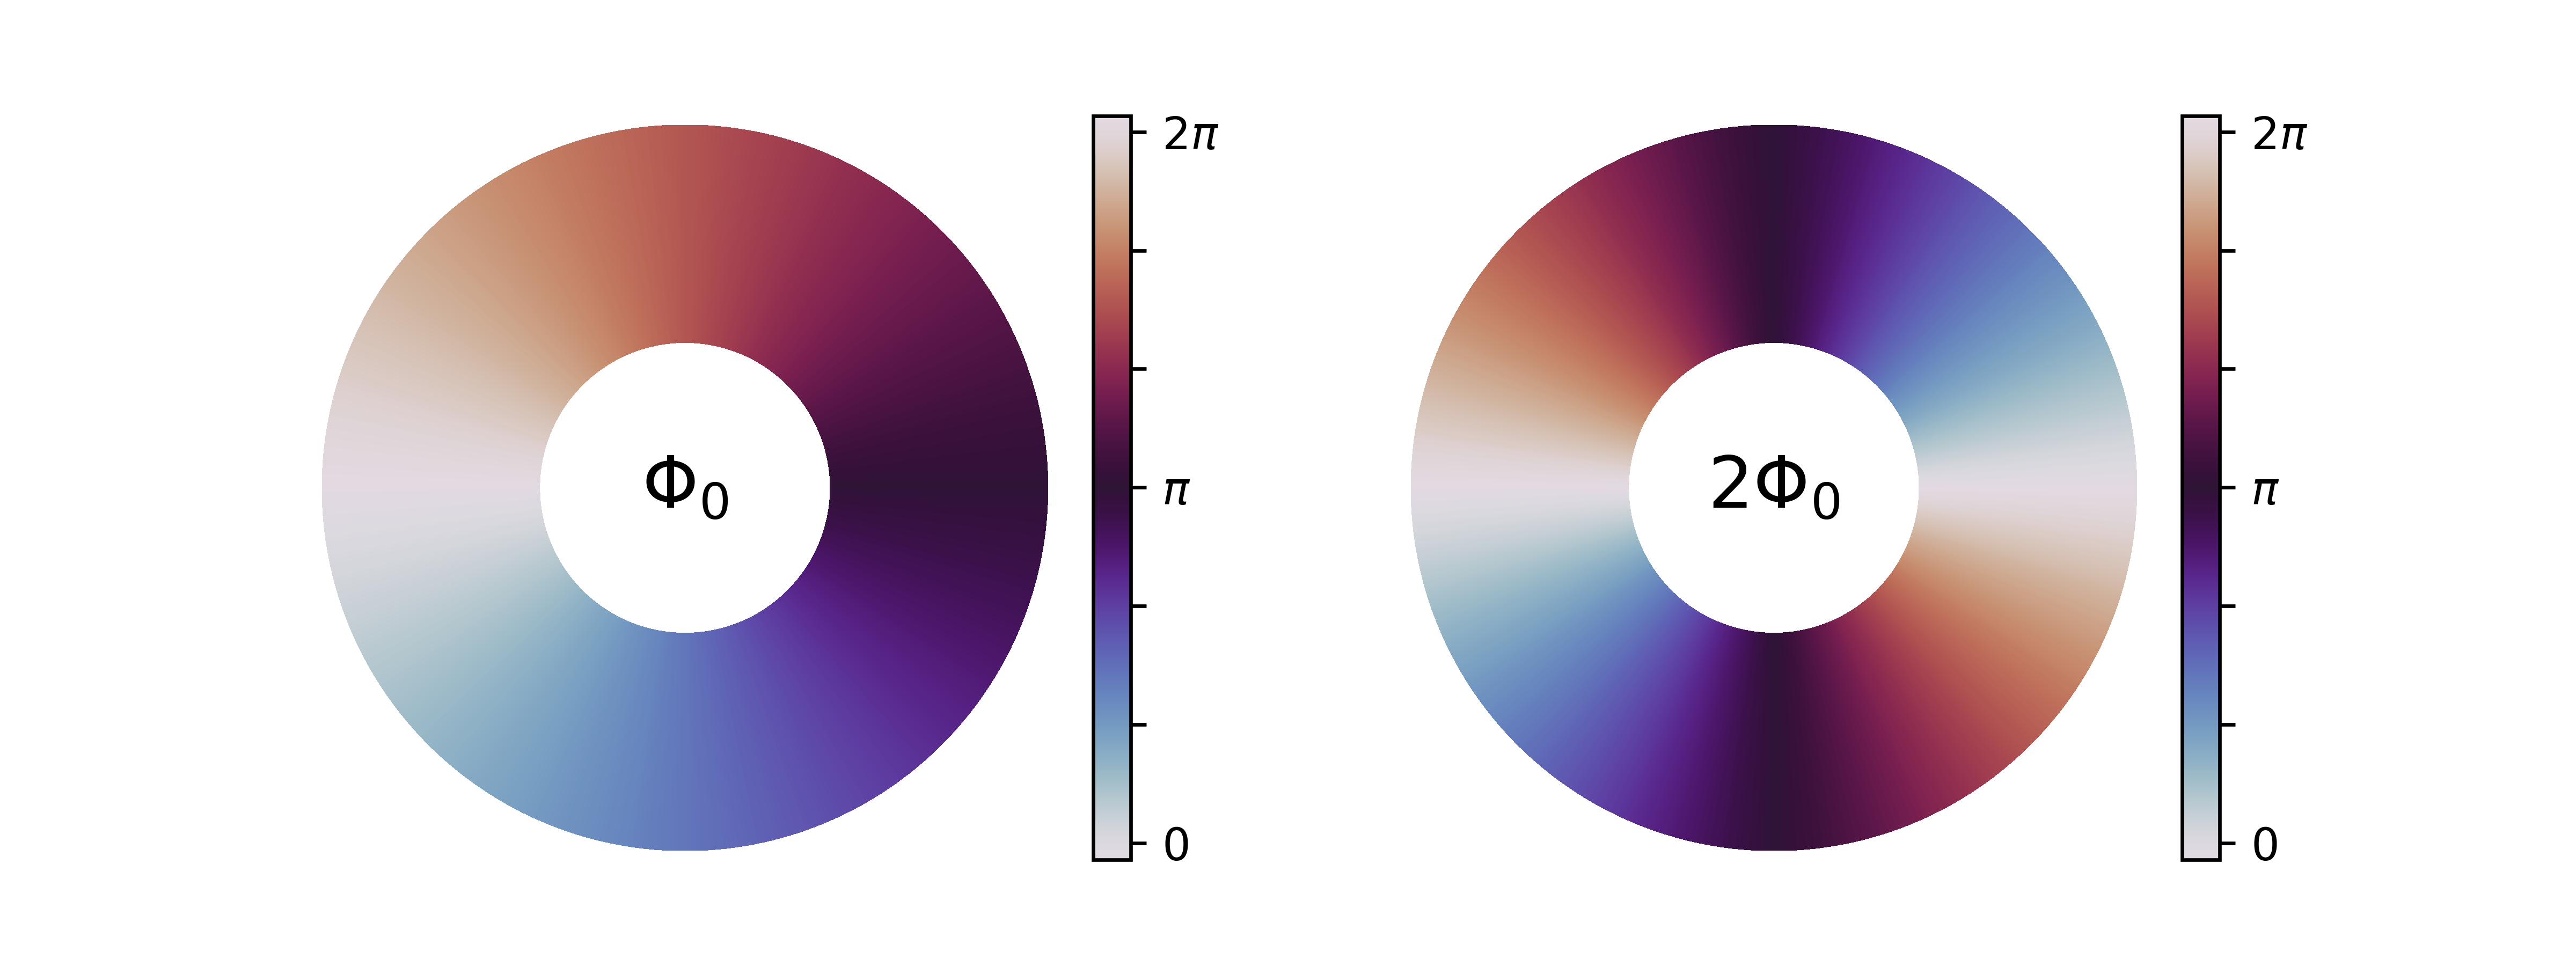
\includegraphics [width=1\textwidth] {coils}
	\caption{Распределение фазы волновой функции в сверхпроводящем кольце для различных значений магнитного потока.  }
	\label{img:coils}
\end{figure}
Квантование потока наглядно показывает, что во многих физических ситуациях, важных при описании сверхпроводниковых цепей, фаза оказывается очень тесно связанной с магнитным потоком. Экспериментально, квантование потока впервые наблюдалось в работе \cite{FluxQuant}  Связь между $\varphi$ и $\Phi$ носит примерно такой же характер, как связь между $n$ и полным зарядом $Q$ сверхпроводящего острова. Действительно, у сверхпроводящего острова к дискретному заряду $Q_n \!=\! n\cdot2e$ добавляется заряд $q\! = \!CV$, наведённый некоторым напряжением $V$ через какую-либо дополнительную ёмкость $C$, и полный заряд равен $Q\!=\!Q_n\!+\!q$. Похожим образом, <<внутренний>> поток $LI_m$, возникающий за счет индуктивного ответа в кольце на внешнее магнитное поле, складывается с внешним потоком $\Phi_{ext}$, и в результате получается дискретный <<полный>> поток $\Phi\!=\!n\Phi_0$. Но как создать какую-либо наведенную непрерывным образом фазу? Оказывается, что при использовании эффекта Джозефсона это становится возможным.
\section{Эффект Джозефсона} 
\subsection{Общие принципы}
Чтобы понять суть эффекта Джозефсона, рассмотрим два объемных сверхпроводника (берега), разделенных слоем диэлектрика. Будем называть такую систему джозефсоновским переходом (или SIS-переходом). Если этот слой достаточно толстый, то берега никак не связаны между собой. Начнем мысленно уменьшать толщину диэлектрического слоя, и рано или поздно возникнет туннельный эффект. Туннелировать могут как отдельные электроны (квазичастицы), так и куперовские пары, существующие независимо для каждого берега. Но куперовские пары имеют удвоенную массу по сравнению с квазичастичными возбуждениями. Поскольку вероятность прохожения барьера экспоненциально падает с ростом массы частицы, то при какой-то толщине $h_1$ барьер станет прозрачным только для квазичастиц, не пропуская куперовские пары. Квазичастицы не формируют конденсат, поэтому такое одноэлектронное туннелирование принципиально не будет отличаться от сходных процессов в нормальных металлах или полупроводниковых структурах. Туннельный ток будет зависеть от плотности состояний, и поэтому будет отличен от нуля только при $V\!>\!2\Delta$, что впервые наблюдалось в работе \cite{GiaeverGap}. Хоть процесс туннелирования куперовских пар весьма маловероятен, но тем не менее, барьер уже достаточно прозрачен, и можно сказать, что волновая функция отдельных электронов из одного берега частично проникает в другой. Продолжим уменьшать толщину диэлектрика. Оказывается, что при некоторой толщине $h_2\!<\!h_1$ возникает когерентность во всей электронной системе. Можно сказать, что куперовские пары образуются из электронов, принадлежащих двум разным металлам одновременно. Эти пары увлекаются в один или другой металл, а направление и  скорость их увлечения зависит от разности сверхпроводящих фаз между берегами. То есть, ненулевой сверхпроводящий ток возникает при $V\!=\!0$. Описанные процессы туннелирования схематично изображены на Рис.\:\ref{img:jj_tunn}. Из качественного рассмотрения может показаться, что одночастичный ток и ток конденсата должны возникать при одинаковой толщине барьера, но в действительности джозефсоновский ток наблюдается при меньшем нормальном сопротивлении, чем одночастичный. Это связано с влиянием тепловых флуктуаций, которые растут с увеличением $R$. Детальное описание можно найти в \cite{Barone}. Покажем, как этот ток зависит от разности фаз.
\begin{figure}
{\centering 
\hfill
\fontsize{22pt}{22pt}\selectfont
\def\svgwidth{3.5in}%
\input{images/JJ_disser.pdf_tex}
\hfill
}
\caption{SIS переход и различные процессы туннелирования через барьер.}
\label{img:jj_tunn}
\end{figure}
\subsection{Токо-фазовое соотношение}

%Прежде чем перейти к описанию эффекта Джозефсона, рассмотрим упрощенную модель электронной системы в сверхпроводнике в представлении зонной структуры. Прежде всего, имеется конденсат куперовских пар, то есть все пары находятся на одном энергетическом уровне, который можно выбрать за нулевой: $E=0$. Если разорвать пару, то возникает 2 квазичастичных возбуждения (электрона) c энергией $E>\Delta$, и если электрон видит частично прозрачный барьер, то он может протунеллировать из сверхпроводника. Также возможен процесс, когда уже имеющийся электрон с другой стороны барьера Вопрос о плотности состояний квазичастиц в зависимости от энергии может быть рассмотрен в теории БКШ, которая дает ответ:


Будем считать, что каждый из берегов имеет собственные состояния конденсата куперовских пар в нем, которые можно описать при помощи макроскопической волновой функции: $\Psi_R\! =\! \sqrt{\rho_R}e^{i\varphi_R}$ и $\Psi_L \!=\! \sqrt{\rho_L}
e^{i\varphi_L}$, где $\rho_R, \rho_L$ --- плотности частиц. Состояние всего конденсата можно искать в виде $\Psi = \Psi_L\ket{L}\!+\!\Psi_R\ket{R}$, что означает, что общий конденсат куперовских пар когерентно распределится так, чтоб минимизировать энергию всей системы. В базисе состояний $\ket{R}, \ket{L}$ гамильтониан системы можно записать в виде:
\begin{equation}
H = E_L\cdot \ket{L}\bra{L} + E_R\cdot \ket{R}\bra{R} + T\cdot\big[ \ket{L} \bra{R}+\ket{R}\bra{L}\big],
\end{equation}
где последний член описывает туннелирование системы как целого и означает, что потенциальный барьер достаточно прозрачен, и некоторые пары из конденсата могут состоять из электронов находящихся по разные стороны от барьера. Теперь можно решить уравнение Шредингера $i\hbar d\Psi/dt\! =\! H\Psi$, распадающееся на два уравнения для амплитуд $\Psi_L$~и~$\Psi_R$: 
\begin{align}
	i\hbar \frac{d\Psi_R}{dt} & =E_R\Psi_R+T\Psi_L, \nonumber \\
    i\hbar \frac{d\Psi_L}{dt} & =E_L\Psi_L+T\Psi_R.
    \label{eq: je_deriv}
\end{align} 
Подставим выражения для $\Psi_L$~и~$\Psi_R$, и получим ответ для плотности сверхпроводящего (джозефсоновского) тока через барьер $J_s={d\rho_R}/{dt}=-{d\rho_L}/{dt}$:
\vspace{-1pt}
\begin{equation}
J=\frac{2T}{\hbar}\sqrt{\rho_R \rho_L}\sin \varphi = J_c \sin \varphi,
\label{eq: cur-phase}
\end{equation}
где $\varphi = \varphi_L-\varphi_R$. Если считать $\rho_L$ и $\rho_R$ константами, что будет справедливо, например, в случае подключения к внешнему источнику тока, то величина $J_c$, называемая плотностью критического тока, зависит только от свойств перехода, а именно от типа сверхпроводника и ширины туннельного барьера. Микроскопическая теория дает следующее выражение для критического тока $I_c$ джозефсоновского перехода в случае нулевой температуры и одинаковых сверхпроводников с $\Delta_L=\Delta_R=\Delta$:
\begin{equation}
I_c = \frac{\pi \Delta}{2eR_n},
\end{equation}
где $R_n$ --- остаточное сопротивление на переходе при $T \ge T_c$. Впервые стационарный эффект Джозефсона наблюдался в работе \cite{StatJosephsonExp}.
Зависимость $J=J(\varphi)$ вида \eqref{eq: cur-phase} характерна не только для туннельного SIS-перехода, но и для многих других типов слабой связи (например, мост Дайема, SNS- и SSeS-переходы \cite{LikharevWL, CPhiR_review}). 
\subsection{Фазо-потоковое соотношение}
Выше было рассмотрено квантование магнитного потока в сплошном кольце. Рассмотрим, как меняется ситуация при прерывании кольца некоторым количеством SIS-переходов ($n$ штук), плоскости которых перпендикуляры плоскости кольца, см. Рис.\:\ref{img:ph-fl}. Будем считать, что внешнее магнитное поле невелико, и можно не учитывать его проникновение в область диэлектрика (которое приводит к необычным эффектам в переходах, см., например, \cite{Schmidt}, \S\:24). Выберем замкнутый контур $C$, пролегающий в глубине кольца, и запишем уравнение \eqref{eq:2GL} с учетом обращающегося в ноль мейсснеровского тока:
\begin{equation}
\label{eq: FFR}
\oint\displaylimits_{C}^{} \mathbf{A} d\boldsymbol{\ell} = \frac{\Phi_0}{2\pi}\oint\displaylimits_{C}^{}\nabla\varphi d\boldsymbol{\ell}
\end{equation}
Правая часть этого выражения содержит интеграл от градиента фазы вдоль контура. Однако, фаза не является непрерывной функцией, а скачкообразно меняется на переходах. Поэтому в таком виде вычислять интеграл нельзя. Разобъем контур $C$ на несколько отрезков кривой $A_iB_i, i=1,\ldots n$, таким образом исключая короткие отрезки контура $C$, лежащие внутри переходов, из контура интегрирования. Будем считать что левый интеграл при этом не изменяется:
\begin{equation}\label{eq:int_cAdl}
\oint\displaylimits_{C}^{} \mathbf{A} d\boldsymbol{\ell} = \sum_{i=1}^{n}\int\displaylimits_{A_i}^{B_i} \mathbf{A} d\boldsymbol{\ell},
\end{equation}
поскольку ширины переходов достаточно малы, а векторный потенциал не имеет никаких особенностей в коротких отрезках контура $C$, лежащих внутри переходов, так как токи и магнитные поля нулевые. Теперь вычислим правый интеграл как:
\begin{equation}
\label{eq:int_phi}
\begin{alignedat}{2}
\oint\displaylimits_{C}^{}\nabla\varphi d\boldsymbol{\ell} = \sum_{i=1}^{n}\int\displaylimits_{A_i}^{B_i}\nabla\varphi d\boldsymbol{\ell} = \sum_{i=1}^{n}\varphi_{B_i}-\varphi_{A_i} & = \\ =\varphi_{A_1} + \sum_{i=1}^{n-1}(\varphi_{A_{i+1}}-\varphi_{B_i}) - \varphi_{B_n} & = 2\pi k + \sum_{i=1}^{n}(\varphi_{A_{i+1}}-\varphi_{B_i}) = \\ 
& =2\pi k + \sum_{i=1}^{n}\delta\varphi_i,
\end{alignedat}
\end{equation}
В предпоследнем равенстве использовано условие однозначности волновой функции в виде $\varphi_{A_1} = \varphi_{A_{n+1}}-2\pi k$. Разности фаз на переходах обозначены как $\delta\varphi_i$. Подставляя \eqref{eq:int_cAdl} и \eqref{eq:int_phi} в \eqref{eq: FFR}, получаем искомое фазо-потоковое соотношение:
\begin{equation}
\label{eq: FFR_final}
\frac{2\pi\Phi}{\Phi_0} = 2\pi k + \sum_{i=1}^{n}\delta\varphi_i.
\end{equation}
Таким образом, поток в таком кольце не квантуется, но однозначно определяется разностями фаз на джозефсоновских переходах. Предположим, например, что джозефсоновские энергии переходов, входящих в кольцо, одинаковы и равны $E_J$, соответственно, равны и критические токи $I_c$. Тогда
\begin{equation}\label{eq: FFR_case}
\frac{2\pi}{\Phi_0}(\Phi_{ext}-LI_c\sin \delta\varphi)= 2\pi k + n\delta\varphi,
\end{equation}
и при заданных $L\text{ и }\Phi_{ext}$ можно найти такие $k \text{ и } \delta\phi$, которые характеризуют разрешенные состояния системы. 
\begin{figure}
	\centering
		\fontsize{22pt}{22pt}\selectfont
		\def\svgwidth{3.5in}%
		\input{images/phase-flux2.pdf_tex}
	\caption{К выводу фазо-потокового соотношения.}
	\label{img:ph-fl}
\end{figure}
%\begin{figure}[ht] 
%	\centering
%	\includegraphics [width=1\textwidth] {coils_jj.png}
%	\caption{Распределение фазы волновой функции в сверхпроводящем кольце для различных значений магнитного потока.}
%	\label{img:coils_JJ}
%\end{figure}
\subsection{Энергия джозефсоновского тока. RSCJ-модель.}
Из уравнений \eqref{eq: je_deriv} можно получить следующее соотношение:
\begin{equation}
\frac{d\varphi}{dt} = \frac{2eV}{\hbar}.
\label{eq: dphidt}
\end{equation}
Таким образом, при конечном напряжении на контакте фаза начинает меняться с течением времени. Это так называемый нестационарный эффект Джохефсона, имеющий множество интересных применений, например генерация высокочастотного тока и создание стандарта напряжения. Используя полученное соотношение, можно рассчитать потенциальную (свободную) энергию, сосредоточенную в переходе:
\begin{equation}
\label{eq:EJ}  
E(\varphi) = \int_{0}^{t}I_sVdt = \int_{0}^{\varphi} I_c\sin \varphi' \frac{\hbar}{2e} {d\varphi'} = E_J(1-\cos\varphi).
\end{equation}
В последнем равенстве учтено что при нулевой фазе ток через переход не течет, и $E(0)=0$. Величина $E_J = {\hbar I_c}/{2e}$ называется \textit{джозефсоновской энергией} перехода. При малых значениях $\varphi$ энергия квадратично зависит от фазы: $E_J\approx E_J \varphi^2/2$, что дает возможность ввести эквивалентную линейную индуктивность перехода $L_{lin} = \Phi_0^2/2\pi I_c$. В более общем случае, джозефсоновская индуктивность зависит от фазы и определяется как $L_J = \Phi_0/(2\pi I_c \cos \varphi)$.
\begin{figure}[ht]
	{\centering
		\hfill
%		\subbottom[List-of-Figures entry][Туннельные процессы в SIS-переходе.\label{img:jj_tunnel}]{%
%			\input{images/JJ_disser.pdf_tex}}
%		\hfill
		\subbottom[List-of-Figures entry][RCSJ-модель перехода.]{%
			\input{images/RSCJ.pdf_tex}}
		\label{img:RCSJ}
		\hfill
		\def\svgwidth{2.2in}
		\subbottom[Частица в потенциале $U(\varphi)$.]{%
			\input{images/washboard.pdf_tex}}
		\label{fig: washboard}
		\hfill
	}
	\caption{RCSJ-модель джозефсоновского туннельного перехода.}
	\label{img:knuth_2}
\end{figure}
До сих пор мы рассматривали лишь энергию сверхпроводящего тока. Однако, для описания нестационарных процессов в реальных туннельных контактах такая модель недостаточна. Необходимо учитывать два дополнительных фактора: квазичастичное туннелирование и значительная емкость между двумя сверхпроводниками, неизбежно возникающая из-за малой толщины диэлектричекой прослойки (несколько десятков межатомных расстояний). Эти аспекты учитываются в феноменологической RCSJ-модели перехода, в которой параллельно с джозефсоновским элементом, энергия которого зависит от фазы согласно \eqref{eq:EJ}, включается эквивалентный резистор $R$, описывающий нормальное сопротивление квазичастичному току, и конденсатор $C$, см.\:Рис.\:\ref{img:RCSJ}. Полный ток через переход в такой схеме можно записать как:
\begin{align}
I &= I_C + I_J + I_R = \frac{\hbar C}{2e} \frac{d^2\varphi}{dt^2}+I_c\sin \varphi+ \frac{\hbar}{2eR}\frac{d\varphi}{dt}, \text{ отсюда получаем:}  \nonumber \\
0 & = m\frac{d^2\varphi}{dt^2} + f \frac{d\varphi}{dt} + \frac{d}{d\varphi}\big(E_J\cos \varphi+E_J\frac{ I}{Ic}\varphi\big), 
\end{align}
где введены обозначения $m=(\hbar/2e)^2 C$ и $f=(\hbar/2e)^2R^{-1}$. Полученное уравнение описывает динамику фазы в переходе как классическое движение частицы массой $m$ в жидкой среде с коэффициентом вязкости $f$ во внешнем потенциале стиральной доски $U(\varphi)=-E_J(\cos \varphi+I\varphi/I_c)$, что схематично отражено на Рис.\:\ref{fig: washboard}. Отметим некоторые характерные особенности динамики системы:
\begin{itemize}
	\item При отсутствии тока потенциал синусоидален, и частица локализуется в потенциальной яме, форма которой близка к параболической, и в этом случае может совершать малые колебания с частотой $\omega_p = (\sqrt{L_{lin}C})^{-1}$, называемой \textit{плазменной частотой перехода}. 
	\item Если увеличивать ток, то наклон потенциала растёт, потенциальная яма становится все более мелкой и пропадает. Частица начинает двигаться и будет разгоняться вдоль стиральной доски, пока не достигнет режима, в котором среднее значение $\langle V \rangle  \propto \langle d\varphi/dt \rangle$ постоянно и отлично от нуля. Характер её замедления при уменьшении тока (наклона) определяется параметром Маккамбера $\beta_c = \omega_p R C$, который показывает обратное число плазменных колебаний, которые система может совершить за время затухания $RC$ (при отсутствии тока).
	\item Если $\beta_c\ll1$, то при уменьшении тока частица практически не замедляется до тех пор, пока наклон не упадет практически до нуля. 
	\item Если $\beta_c \gg 1$, то частица замедляется довольно значительно, так как трение играет существенную роль в её движении и скорость движения вдоль стиральной доски определяется средним наклоном. Полная остановка, однако, также произойдет лишь при $I=0$.
\end{itemize}
Перечисленные особенности находят подтверждение при измерении ВАХ переходов, полученных при фиксированном внешнем токе $I$, см., например, \cite{Schmidt}. 
Подведем итог классическому описанию джозефсоновского перехода. В зависимости от выбранного режима работы, такой переход может вести себя как нелинейный осциллятор, нелинейная индуктивность, зависящая от времени, либо демонстрировать еще более сложное поведение. Это делает его весьма интересным элементом даже с точки зрения классической схемотехники. Еще более нетривиальные эффекты возникают в том случае, если рассматривать разность фаз на переходе как квантовую степень свободы, которые мы кратко опишем далее. 
\section{Квантование электрических цепей}
Как было сказано выше, при квантовом описании какой-либо сверхпроводящей системы число пар $\hat{n}$ на сверхпроводящем острове и фаза $\hat{\varphi}$ на этом острове могут рассматриваться как сопряженные переменные: $[\hat{\varphi}, \hat{n}]=i$. Возбуждения коллективной квантовой степени свободы при определенных условия оказываются самыми низкоэнергетическими (ниже 10 ГГц), и потому есть возможность экспериментально работать только с ними. В сверхпроводниках минимальная энергия одноэлектронного возбуждения не может быть меньше $2\Delta$, например, для алюминия имеем $2\Delta=3.52 k_b T_c\approx h\cdot80$ ГГц. Можно показать \cite{girvin2011circuit}, что частоты объемных плазменных колебаний попадают в терагерцовый диапазон, и поэтому их также можно исключить из рассмотрения. Фактически, мы будем иметь дело с бездисперсионными коллективными плазменными возбуждениями, и именно эти моды в итоге будут квантоваться. 

Опишем общий подход к квантованию СКЦ \cite{vool2017introduction}. Будем рассматривать некоторую систему, состоящую из набора сверхпроводящих островов. Острова могут быть связаны взаимными емкостями и индуктивностями. Кроме того, некоторые из них могут образовывать джозефсоновскую связь. Поэтому, достаточно общим является представление такой системы в качестве электрической цепи, в которой имеются три типа элементов: емкости, индуктивности и джозефсоновские элементы (нелинейные индуктивности)\footnote[1]{Совсем недавно \cite{astafiev2012coherent} показана возможность создания т.н. центра когерентного квантового проскальзывания фазы, который является емкостным аналогом джозефсоновского перехода. Однако, создание квантовых цепей из таких элементов еще не вполне отработано. Их описание выходит за рамки данной работы.}. Как и в электротехнической цепи, в такой системе нужно подходящим образом выбрать некоторые независимые степени свободы, с помощью которых можно описать как классическую, так и квантовую динамику системы. Последовательность действий квантования системы состоит из следующих шагов:
\begin{enumerate}
\item Изобразим эквивалентную электрическую схему цепи. Схема будет состоять из N узлов (точек), связанных произвольным количеством элементов-двуполюсников, которые мы будем называть ребрами. Мысленно выделим емкостную и индуктивную части в общей схеме цепи. Поскольку любой реальный элемент имеет конечные размеры, и следовательно, паразитную емкость, то можно считать, что между каждой парой узлов включена емкость, и притом единственная. Среди всех узлов можно выделить \textit{активные} узлы, к которым подсоединены как емкостные, так и индуктивные элементы, и \textit{пассивные} узлы, к которым подсоединены только емкости.


\item Для каждого ребра введем величину $\Phi(t)=\int_{-\infty}^{t} v(t')dt'$, которую можно назвать магнитным потоком через ребро. Считается, что напряжение $v(-\infty)=0$ и плавно включается со временем. Тогда емкостную энергию можно записать как $C\dot{\Phi}^2/2$, что соответствует кинетической энергии частицы с кординатой $\Phi$. Для индуктивности эта величина в точности совпадает с запасённым в ней магнитным потоком, и индуктивная энергия $(\Phi-\widetilde{\Phi})^2/2L$ играет роль потенциальной энергии, где $\widetilde{\Phi}$ --- некоторый внешний поток. 
\item Выберем один из активных узлов емкостной подсистемы в качестве заземленного узла, и выберем только те емкости, которые единственным образом соединяют земляной узел со всеми остальными узлами подсистемы. Эти емкости составят \textit{остовное дерево} $T$. Тогда для любого другого узла $n$ можно ввести т.н. \textit{узловой поток} $\phi_n$, который равен сумме потоков всех емкостей, через которые нужно пройти от земляного узла до узла $n$. Связь между потоком через некоторое ребро $\Phi_b$ и потоками через узлы этого ребра $\phi_n, \phi_{n'}$ даётся соотношением:
\begin{equation}\label{eq: Phiphi}
\begin{aligned}
	\Phi_{b\in T} &= \phi_n-\phi_{n'}, \\
	\Phi_{b\notin T} &= \phi_n-\phi_{n'} + \widetilde{\Phi}_b,
\end{aligned}
\end{equation}
где внешний поток ${\Phi}_b$ учитывается в том случае, когда добавление ветви $b$ образует индуктивную петлю.
\item Используя соотношения \eqref{eq: Phiphi}, запишем полную энергию индуктивной и емкостной подсистемы через переменные $\vec{\phi}=(\phi_1\ldots\phi_N)^T$.  Энергия индуктивной подсистемы примет вид:
\begin{equation}
E_L(\vec{\phi}) = \frac{1}{2}{\vec{\phi}^{\mathsmaller T}} \mathbf{L^{-1}}\vec{\phi} + \sum_b \frac{\phi_n-\phi_{n'}}{L_b}\widetilde{\Phi}_b.
\end{equation}
Первое слагаемое представляет собой вклад в энергию непосредственно от индуктивностей. Матрица индуктивности $\mathbf{L}$ размера $(N-1)\!\times\!(N-1)$ симметричная и сконструирована следующим образом: недиагональные элементы $(i,j)$ равны $-\sum L_{ij}$, где $L_{ij}$ - все индуктивности, соединяющие узлы $i$ и $j$; диагональные же элементы равны сумме всех недиагональных элементов на соответствующей строке (или в столбце), взятой с противоположным знаком. Второе слагаемое --- это энергия каждой индуктивности, которая находится в ветви с внешним потоком $\widetilde{\Phi}_b$. Энергия емкостной подсистемы примет вид:
\begin{equation}
E_C(\dot{\vec{\phi}})= \frac{1}{2} {\dot{\vec{\phi}}^{\mathsmaller T}} \mathbf{C^{-1}} \dot{\vec{\phi}}
\end{equation}
где матрица емкости $\mathbf{C}$ строится аналогично матрице индуктивности.
\item Полученные выражения позволяют записать лагранжиан системы $\mathcal{L} = E_C-E_L$ и найти классические уравнения движения $\frac{d}{dt}\frac{\partial\mathcal{L}}{\partial\dot{\phi_n}}=\frac{\partial\mathcal{L}}{\partial{\phi_n}}$. Поскольку нас интересует квантовое описание системы, необходимо найти обобщенные импульсы $q_n = \partial\mathcal{L}/\partial{\dot\phi_n}$,  и записать гамильтониан $H = q_n\phi_n-\mathcal{L}$. Сколько независимых степеней свободы будет иметь система? Чтобы ответить на этот вопрос, необходимо заметить, что для любого пассивного узла $\partial \mathcal{L}/\partial{\phi_n}=0$, а поэтому $q_n$ является константой, и фактически, даннная степень свободы вырождена. Таким образом, если число активных узлов $P$, то полное число степеней свободы $P-1$.
\item Заменяя координаты (узловые потоки) и импульсы (узловые заряды) на сопряженные операторы $\phi\rightarrow\hat{\phi}$~и~$q\rightarrow\hat{q} = -i\hbar\frac{\partial}{\partial \phi}$, получаем гамильтониан квантовой цепи. Далее можно найти стационарные состояния, их энергии, матричные элементы переходов, и описать динамику системы.
\end{enumerate}
Далее мы рассмотрим некоторые бавзовые типы СКЦ. Как правило, они достаточно просты, и можно записать гамильтониан практически сразу, без предварительных шагов. Однако, следование общему формализму квантования необходимо для правильного описания более сложных цепей со многими степенями свободы. 
   
\section{Типы кубитов}
Базовые типы СКЦ, далее просто кубитов - это зарядовый кубит, фазовый кубит, потоковый кубит, трансмон и вч-СКВИД. Кратко опишем свойства каждого из этих кубитов.
\subsection{Зарядовый кубит}
	\begin{figure}[b]
		{\centering
			\hfill
			\def\svgwidth{2.2in}
			\fontsize{19pt}{19pt}\selectfont
			\subbottom[List-of-Figures entry][Схема кубита\label{img: CPB_scheme}]{%
				\input{images/CPB_qubit.pdf_tex}}
			\hfill
			\def\svgwidth{2.2in}
			\fontsize{19pt}{19pt}\selectfont
			\subbottom[Спектр кубита]{%
				\input{images/CPB_qubit.pdf_tex}}
			\label{img: CPB_spectrum}
			\hfill
		}
		\caption{Зарядовый кубит}
		\label{img: CPB}
		
	\end{figure}
Зарядовый кубит, или <<ящик>> для куперовских пар - это система, представляющая из себя джозефсоновский переход с энергией $E_J$, последовательно соединённый с емкостью. Эквивалентная схема такого кубита изображена на Рис.\ref{img: CPB}\subcaptionref*{img: CPB_scheme}. Образуется изолированный остров (выделен синим цветом), и если его емкость достаточно мала, то изменение числа куперовских пар на единицу сильно меняет энергию системы.  Введем зарядовую энергию конденсатора $E_C = 4e^2/C$; она включает в себя всю эффективную емкость острова, в т.ч. джозефсоновскую емкость. Также к острову подключен внешний источник, который может создавать наведенный заряд $n_g = C_gV_g/2e$.   Остовное дерево и земля выбираются тривиально, и понятно, что единственная степень свободы задается операторами фазы $\hat{\varphi}_1\!=\!2\pi/\Phi_0\!\cdot\!\hat{\phi}_1$ и заряда $\hat{n}_1\!=\!\hat{q}_1/2e$.~Гамильтониан системы имеет вид:

\subsection{Фазовый кубит}
\subsection{Потоковый кубит}
\subsection{Трансмон}
\subsection{вч-СКВИД}